\usepackage{graphicx}
\usepackage{hyperref}
\title{To Catch a Falling Star}
\subtitle{Searching for X-Ray Flares in Archival Chandra \& XMM Images of Galaxy Clusters}
\author{Matthew P. Wampler-Doty}
\date{}
\begin{document}
\maketitle
\frame{\frametitle{Table of Contents}\tableofcontents}
\section{Overview}
\subsection{How Do Astronomers Analyze Images?}
\section{Detecting Flares}
\subsection{Retrieving Archive Observation Data}
\subsection{Agglomerating Observations by Position}

\begin{frame}[allowframebreaks]
\frametitle{Hierarchical Agglomerative Clustering Overview}
\begin{itemize}
	\item \emph{Hierarchical agglomerative clustering} successively merges pairs of clusters with their \emph{closest} neighbor, based on a measure $D$, until there is nothing left to merge
	\item We use \emph{complete-linkage} as our measure -- that is, we say
\begin{eqnarray*}
  D (X, Y) & = & \underset{y \in Y}{\underset{x \in X}{\max}} (\delta (x, y))
\end{eqnarray*}
	where:
	\begin{itemize}
		\item $\delta(x,y)$ is some distance measure of $x$ and $y$
		\item $X$ and $Y$ are clusters
	\end{itemize}
	\item Efficient $O(n^2)$ algorithm used:
	\url{http://math.stanford.edu/~muellner/fastcluster.html}
\end{itemize}
\framebreak
\begin{itemize}
	\item Same technique used in \emph{computational phylogenics}
\end{itemize}
\begin{figure}[h,b]
\centering
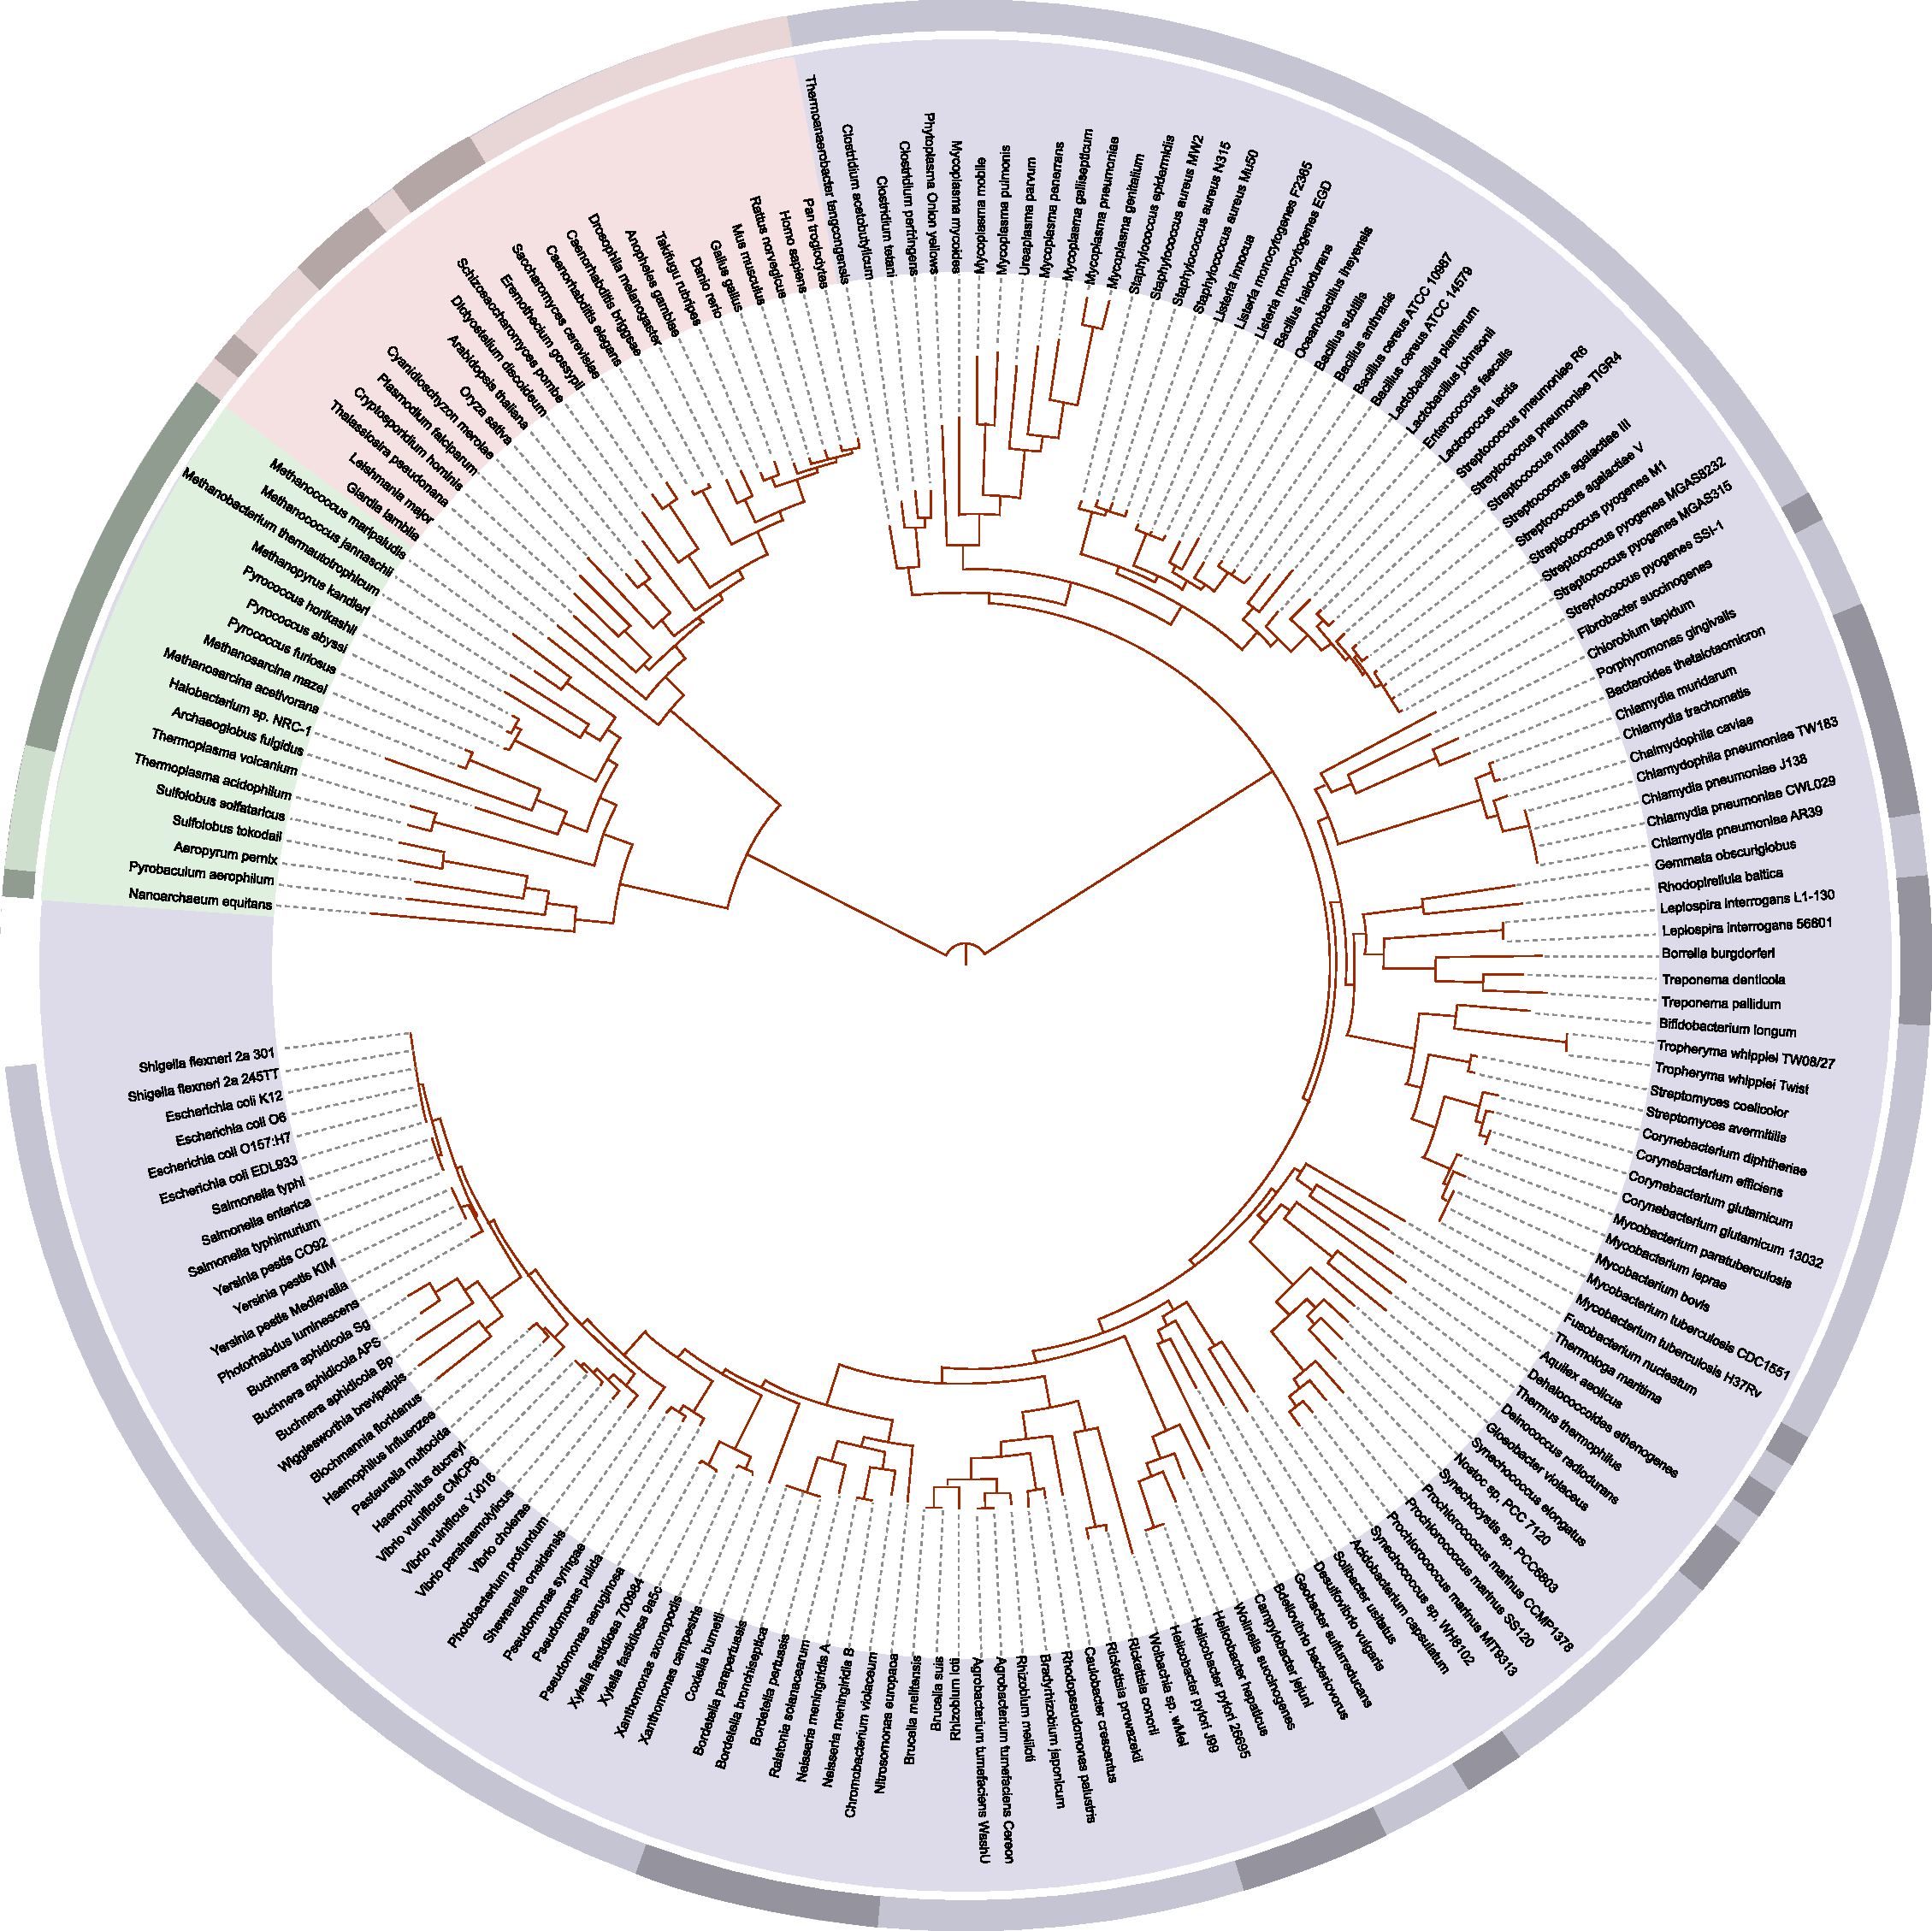
\includegraphics[width=0.6\textwidth]{Tree-of-life-SVG}
\end{figure}
FIXME: Cite Wikipedia?
	
\framebreak
\begin{itemize}
	\item Define $\delta$ by \emph{Great-circle distance}, which is given by \emph{Vincenty's Formula}:
	\begin{eqnarray*}
  \delta (\langle \phi_s, \theta_s \rangle, \langle \phi_f, \theta_f \rangle)
  & = & \arctan \left( \frac{\sqrt{\left( \cos \phi_f \sin \Delta
  \theta \right)^2 + \left( \cos \phi_s \sin \phi_f - \sin \phi_s \cos \phi_f
  \cos \Delta \theta \right)^2}}{\sin \phi_s \sin \phi_f + \cos \phi_s \cos
  \phi_f \cos \Delta \theta} \right)
	\end{eqnarray*}
where:
	\begin{itemize}
	\item $\Delta \theta$ is $\theta_s-\theta_f$
	\item Implemented using \texttt{atan2} in Python (avoids numerical instability and cases where denominator is zero)
	\end{itemize}
\end{itemize}
\end{frame}

\begin{frame}
\frametitle{Vincenty's Formula}

\end{frame}

\begin{frame}
\frametitle{First Slide}
Contents of the first slide
\end{frame}
\begin{frame}
\frametitle{Second Slide}
Contents of the second slide
\end{frame}
\end{document}
